\documentclass[aspectratio=169]{beamer}
\usepackage{lmodern}
%\usetheme{Madrid}
%\usecolortheme{giantoak}
\newcommand*\oldmacro{}
\let\oldmacro\insertshorttitle
\renewcommand*\insertshorttitle{\oldmacro\hfill\insertframenumber\,/\,\inserttotalframenumber}
\usepackage[framemethod=tikz]{mdframed}

%\usepackage{beamerthemesplit}
\usepackage{textpos}
\usepackage{pgf}
\usepackage{ulem}
%\logo{\pgfputat{\pgfxy(0,-.4)}{\pgfbox[right,base]{\includegraphics[height=1.0cm]{logo.jpg}}}}
%\newcommand{\nologo}{\setbeamertemplate{logo}{}}
\usepackage{booktabs}
\usepackage{graphicx}
\theoremstyle{principle}
\newtheorem*{principle}{Design Principle}


\titlegraphic{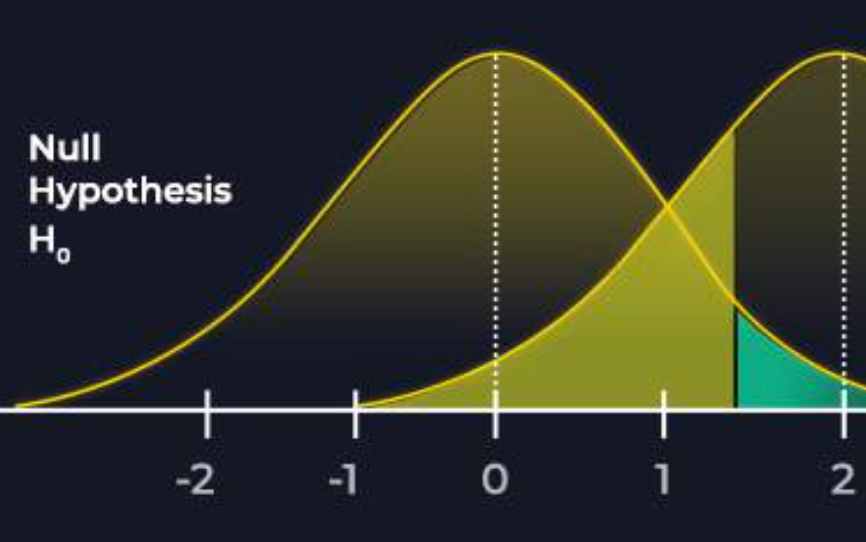
\includegraphics[width=1.0\paperwidth]{distros.png}}

\title{Amendments}
%\author[Jeremy Kedziora]{Wind Data Science Team\\
%\small{Uptake}}
\date{}

\begin{document}

%{
%%\nologo
%\begin{frame}
%    \maketitle
%\end{frame}
%}
%pages 1-7, 8-9, 14-15.


{
%  \usebackgroundtemplate{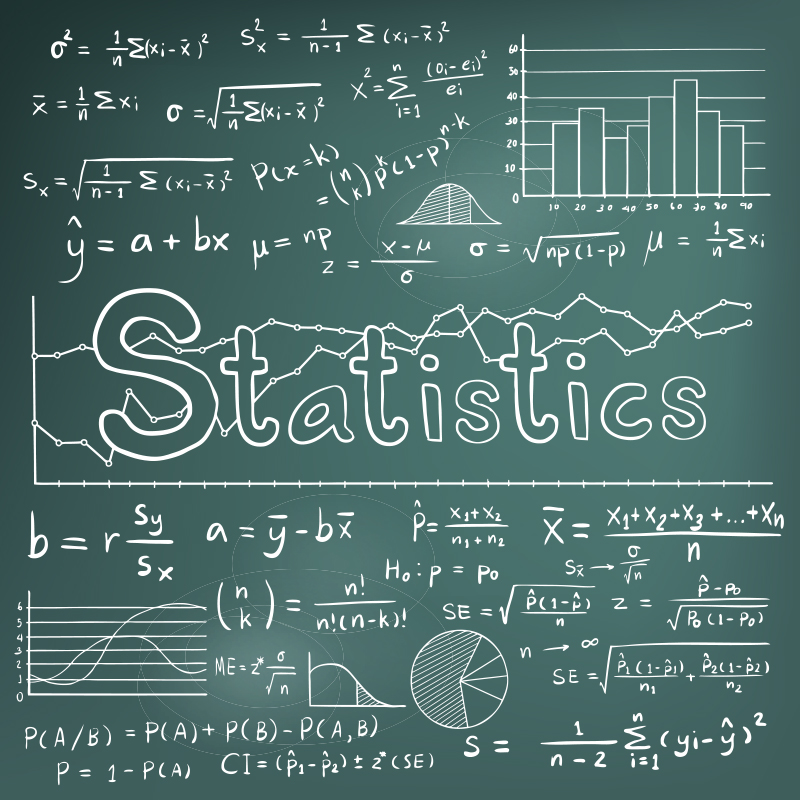
\includegraphics[width=1.0\paperwidth]{statistics-review.jpg}}
  \usebackgroundtemplate{
\includegraphics[scale=0.5]{pretty_data.png}}
  \begin{frame}[plain]
  
\begin{mdframed}[tikzsetting={draw=white,fill=white,fill opacity=0.6,draw opacity=0.4,
               line width=0pt},backgroundcolor=none,leftmargin=20,
               rightmargin=20,innertopmargin=4pt]
\begin{center}
\Huge \textbf{Problems with Linear Regression}
\end{center}
\end{mdframed}

  \end{frame}
}

%most reliant on human cognition
%limited only by cognition
%hypothesis generating scheme often functioning as a gateway into more statistical analysis

%%@@@@@@@@@@@@@@@@@@@@@@@@@@@@@@@@@@@@@@@@@@@@@@@@@
%\begin{frame}
%\frametitle{Napoleon's Progress}
%\begin{center}
%
\includegraphics[scale=0.4]{experiment.png}
%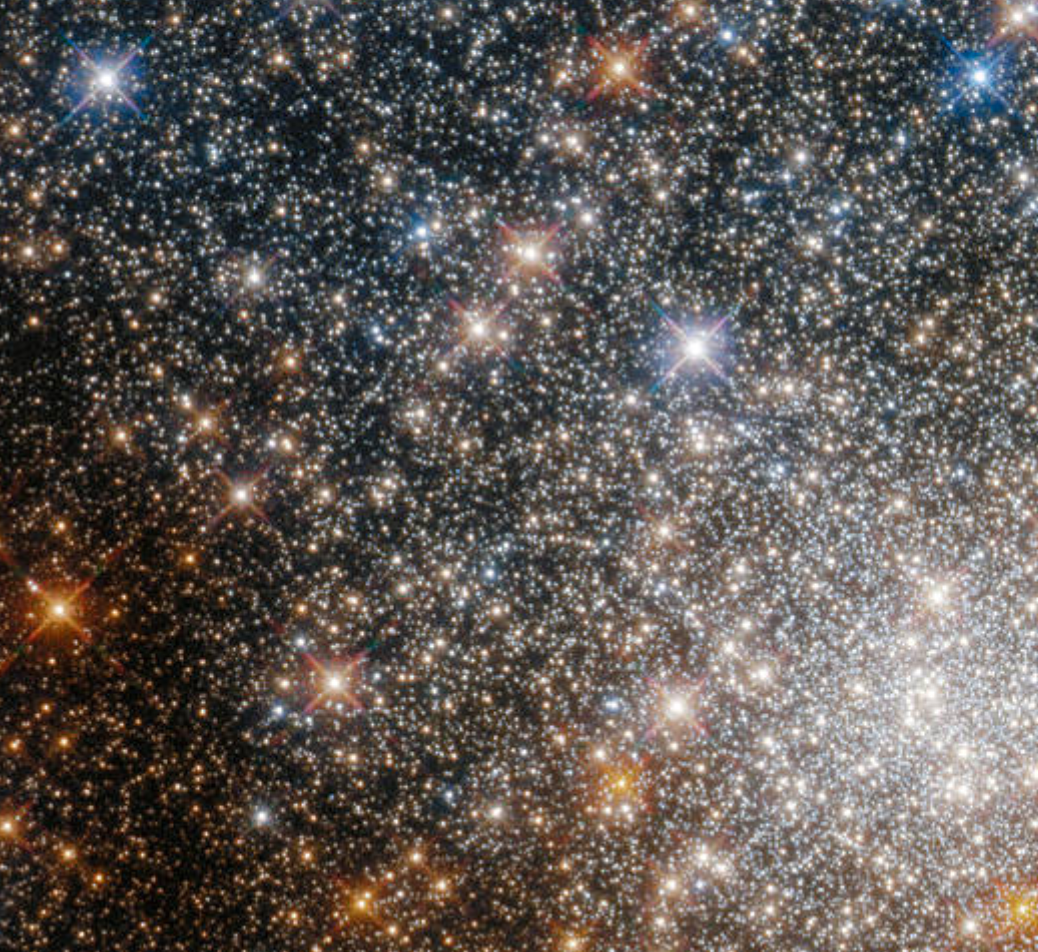
\includegraphics[scale=0.35]{stars.png}
%\end{center}
%
%\end{frame}

%@@@@@@@@@@@@@@@@@@@@@@@@@@@@@@@@@@@@@@@@@@@@@@@@@
\begin{frame}
\frametitle{Today:}

\begin{itemize}
\item Define six major problems analysts using regression run into;
\bigskip
\bigskip
\bigskip

\item Understand what their effects will be on your regression.

\end{itemize}

\end{frame}

%@@@@@@@@@@@@@@@@@@@@@@@@@@@@@@@@@@@@@@@@@@@@@@@@@
\begin{frame}
\frametitle{So far, we've used linear regression to:}

\begin{enumerate} 
\item Model a linear relationship between dependent variable $y$ and independent variable $x$:
\begin{align*}
y = \beta_0 + \beta_1x + \varepsilon;
\end{align*}

\item Model a linear relationship between dependent variable $y$ and many independent variables $x_1,x_2,x_3,\hdots$:
\begin{align*}
y = \beta_0 + \beta_1x_1 + \beta_2x_2 + \beta_3x_3 + \hdots + \varepsilon;
\end{align*}

\item Model a NON-linear relationship between dependent variable $y$ and many independent variables $x$:
\begin{align*}
y = \beta_0 + \beta_1x_1 + \beta_2x_1^2 + \hdots + \varepsilon;
\end{align*}

\item Model relationships between independent variables:
\begin{align*}
y = \beta_0 + \beta_1x_1 + \beta_2x_2 + \beta_{12}x_1x_2 + \varepsilon;
\end{align*}

\end{enumerate}

\end{frame}

%@@@@@@@@@@@@@@@@@@@@@@@@@@@@@@@@@@@@@@@@@@@@@@@@@
\begin{frame}
\frametitle{Reminder: Assumptions of Linear Regression}

\begin{enumerate}
\item Dependent variable is a \textbf{linear} function of independent variables plus noise;
\begin{align*}
y = \beta_0 + \beta_1x_1 + \beta_2x_2 + \hdots + \beta_mx_m + \varepsilon
\end{align*}
\begin{itemize}
\item[]\color{white}Violated by: selecting on the dep var, model specification, endogeneity;
\end{itemize}
\bigskip

\item Independent variables are not related to each other -- \textbf{no multicollinearity};
\begin{itemize}
\item[]\color{white}Violated by: Multicollinearity between indp vars;
\end{itemize}
\bigskip

\item Independent variables have \textbf{no measurement error};
\begin{itemize}
\item[]\color{white}Violated by: Measurement error of indp vars;
\end{itemize}
\bigskip

\item Noise term is a random variable following the \textbf{normal distribution};
\begin{itemize}
\item[]\color{white}Violated by: Heteroscedasticity.
\end{itemize}

\end{enumerate}

\end{frame}

%@@@@@@@@@@@@@@@@@@@@@@@@@@@@@@@@@@@@@@@@@@@@@@@@@
\begin{frame}
\frametitle{Reminder: Assumptions of Linear Regression}

\begin{enumerate}
\item Dependent variable is a \textbf{linear} function of independent variables plus noise;
\begin{align*}
y = \beta_0 + \beta_1x_1 + \beta_2x_2 + \hdots + \beta_mx_m + \varepsilon
\end{align*}
\begin{itemize}
\item Violated by: selecting on the dep var, model specification, endogeneity;
\end{itemize}
\bigskip

\item Independent variables are not related to each other -- \textbf{no multicollinearity};
\begin{itemize}
\item[]\color{white}Violated by: Multicollinearity between indp vars;
\end{itemize}
\bigskip

\item Independent variables have \textbf{no measurement error};
\begin{itemize}
\item[]\color{white}Violated by: Measurement error of indp vars;
\end{itemize}
\bigskip

\item Noise term is a random variable following the \textbf{normal distribution};
\begin{itemize}
\item[]\color{white}Violated by: Heteroscedasticity.
\end{itemize}

\end{enumerate}

\end{frame}

%@@@@@@@@@@@@@@@@@@@@@@@@@@@@@@@@@@@@@@@@@@@@@@@@@
\begin{frame}
\frametitle{Reminder: Assumptions of Linear Regression}

\begin{enumerate}
\item Dependent variable is a \textbf{linear} function of independent variables plus noise;
\begin{align*}
y = \beta_0 + \beta_1x_1 + \beta_2x_2 + \hdots + \beta_mx_m + \varepsilon
\end{align*}
\begin{itemize}
\item Violated by: selecting on the dep var, model specification, endogeneity;
\end{itemize}
\bigskip

\item Independent variables are not related to each other -- \textbf{no multicollinearity};
\begin{itemize}
\item Violated by: Multicollinearity between indp vars;
\end{itemize}
\bigskip

\item Independent variables have \textbf{no measurement error};
\begin{itemize}
\item[]\color{white} Violated by: Measurement error of indp vars;
\end{itemize}
\bigskip

\item Noise term is a random variable following the \textbf{normal distribution};
\begin{itemize}
\item[]\color{white} Violated by: Heteroscedasticity.
\end{itemize}

\end{enumerate}

\end{frame}

%@@@@@@@@@@@@@@@@@@@@@@@@@@@@@@@@@@@@@@@@@@@@@@@@@
\begin{frame}
\frametitle{Reminder: Assumptions of Linear Regression}

\begin{enumerate}
\item Dependent variable is a \textbf{linear} function of independent variables plus noise;
\begin{align*}
y = \beta_0 + \beta_1x_1 + \beta_2x_2 + \hdots + \beta_mx_m + \varepsilon
\end{align*}
\begin{itemize}
\item Violated by: selecting on the dep var, model specification, endogeneity;
\end{itemize}
\bigskip

\item Independent variables are not related to each other -- \textbf{no multicollinearity};
\begin{itemize}
\item Violated by: Multicollinearity between indp vars;
\end{itemize}
\bigskip

\item Independent variables have \textbf{no measurement error};
\begin{itemize}
\item Violated by: Measurement error of indp vars;
\end{itemize}
\bigskip

\item Noise term is a random variable following the \textbf{normal distribution};
\begin{itemize}
\item[]\color{white} Violated by: Heteroscedasticity.
\end{itemize}

\end{enumerate}

\end{frame}

%@@@@@@@@@@@@@@@@@@@@@@@@@@@@@@@@@@@@@@@@@@@@@@@@@
\begin{frame}
\frametitle{Reminder: Assumptions of Linear Regression}

\begin{enumerate}
\item Dependent variable is a \textbf{linear} function of independent variables plus noise;
\begin{align*}
y = \beta_0 + \beta_1x_1 + \beta_2x_2 + \hdots + \beta_mx_m + \varepsilon
\end{align*}
\begin{itemize}
\item Violated by: selecting on the dep var, model specification, endogeneity;
\end{itemize}
\bigskip

\item Independent variables are not related to each other -- \textbf{no multicollinearity};
\begin{itemize}
\item Violated by: Multicollinearity between indp vars;
\end{itemize}
\bigskip

\item Independent variables have \textbf{no measurement error};
\begin{itemize}
\item Violated by: Measurement error of indp vars;
\end{itemize}
\bigskip

\item Noise term is a random variable following the \textbf{normal distribution};
\begin{itemize}
\item Violated by: Heteroscedasticity.
\end{itemize}

\end{enumerate}

\end{frame}

%@@@@@@@@@@@@@@@@@@@@@@@@@@@@@@@@@@@@@@@@@@@@@@@@@
\begin{frame}
\frametitle{Problem 0: Selecting on the dependent variable}

Suppose you are an analyst trying to understand the effect of a certain chemical on mortality.  You collect a sample of deceased persons and you observe that every single one of them was exposed to the chemical in large quantities.  What do you conclude?\\
\bigskip
\color{white}What if I now tell you the chemical is water?

\end{frame}

%%@@@@@@@@@@@@@@@@@@@@@@@@@@@@@@@@@@@@@@@@@@@@@@@@@
%\begin{frame}
%\frametitle{Problem 0: Selecting on the dependent variable}
%
%Suppose you are an analyst trying to understand the effect of a certain chemical on mortality.  You collect a sample of deceased persons and you observe that every single one of them was exposed to the chemical in large quantities.  What do you conclude?\\
%\bigskip
%What if I now tell you the chemical is water?
%
%\end{frame}

%@@@@@@@@@@@@@@@@@@@@@@@@@@@@@@@@@@@@@@@@@@@@@@@@@
\begin{frame}
\frametitle{Problem 0: Selecting on the dependent variable}

\begin{itemize}
\item \textbf{Selecting on the dependent variable} $=$ collecting only one value of $y$ when making the data;
\bigskip
\bigskip

\item \textbf{Effect}: well, you can't run linear regression, and any inferences you try to draw will be unrelated to the data;
\bigskip
\bigskip

\item \textbf{Fix}: collect more data.
\end{itemize}

\end{frame}

%@@@@@@@@@@@@@@@@@@@@@@@@@@@@@@@@@@@@@@@@@@@@@@@@@
\begin{frame}
\frametitle{Problem 1: Model Specification}
\begin{itemize}
\item \textbf{Model specification} $=$ which independent variables you choose to include -- leaving out an independent variable out that should be there is called \textbf{omitted variable bias};
\bigskip
\bigskip

\item \textbf{Effect}: the independent variable effects (the $\beta$'s) that linear regression estimates will be wrong;
\bigskip
\bigskip

\item \textbf{Fix}: theorizing about why variables are/not included, advanced techniques.
\end{itemize}
\end{frame}

%@@@@@@@@@@@@@@@@@@@@@@@@@@@@@@@@@@@@@@@@@@@@@@@@@
\begin{frame}
\frametitle{Problem 1: Model Specification}
\begin{itemize}
\item True relationship between $y$ and $x$'s is:
\begin{align*}
y = 1 + 2x_1 - x_2 + \varepsilon;
\end{align*}
\item[]\color{white} Suppose we omit $x_2$:
\end{itemize}

% latex table generated in R 4.1.1 by xtable 1.8-4 package
% Wed Nov  2 10:31:06 2022
\begin{table}[ht]
\centering
\begin{tabular}{rrrrr}
  \hline
  \hline
 & Estimate & Std. Error & t value & Pr($>$$|$t$|$) \\ 
  \hline
    \hline
(Intercept) & 0.9623 & 0.0317 & 30.40 & 0.0000 \\ 
  x1 & 2.0401 & 0.1030 & 19.80 & 0.0000 \\ 
  x2 & -1.0055 & 0.0322 & -31.19 & 0.0000 \\ 
   \hline
      \hline
\end{tabular}
\end{table}

\end{frame}

%@@@@@@@@@@@@@@@@@@@@@@@@@@@@@@@@@@@@@@@@@@@@@@@@@
\begin{frame}
\frametitle{Problem 1: Model Specification}
\begin{itemize}
\item True relationship between $y$ and $x$'s is:
\begin{align*}
y = 1 + 2x_1 - x_2 + \varepsilon;
\end{align*}
\item Suppose we omit $x_2$:
\end{itemize}

% latex table generated in R 4.1.1 by xtable 1.8-4 package
% Wed Nov  2 10:33:07 2022
\begin{table}[ht]
\centering
\begin{tabular}{rrrrr}
  \hline
  \hline
 & Estimate & Std. Error & t value & Pr($>$$|$t$|$) \\ 
  \hline
    \hline
(Intercept) & 0.9698 & 0.0445 & 21.81 & 0.0000 \\ 
  x1 & -0.9945 & 0.0475 & -20.95 & 0.0000 \\ 
   \hline
      \hline
      &&&&\\
\end{tabular}
\end{table}

\end{frame}

%@@@@@@@@@@@@@@@@@@@@@@@@@@@@@@@@@@@@@@@@@@@@@@@@@
\begin{frame}
\frametitle{Problem 2: Multicollinearity}

\begin{columns}
\begin{column}{0.5\textwidth}

\begin{itemize}
\item \textbf{Multicollinearity} $=$ two (or more) independent variables correlated with each other;
\bigskip
\bigskip

\item \textbf{Effect}: the independent variable effects (the $\beta$'s) that linear regression estimates will be wrong;
\bigskip
\bigskip

\item \textbf{Fix}: drop one of the independent variables, advanced techniques.

\end{itemize}

\end{column}
\begin{column}{0.5\textwidth}
\begin{center}
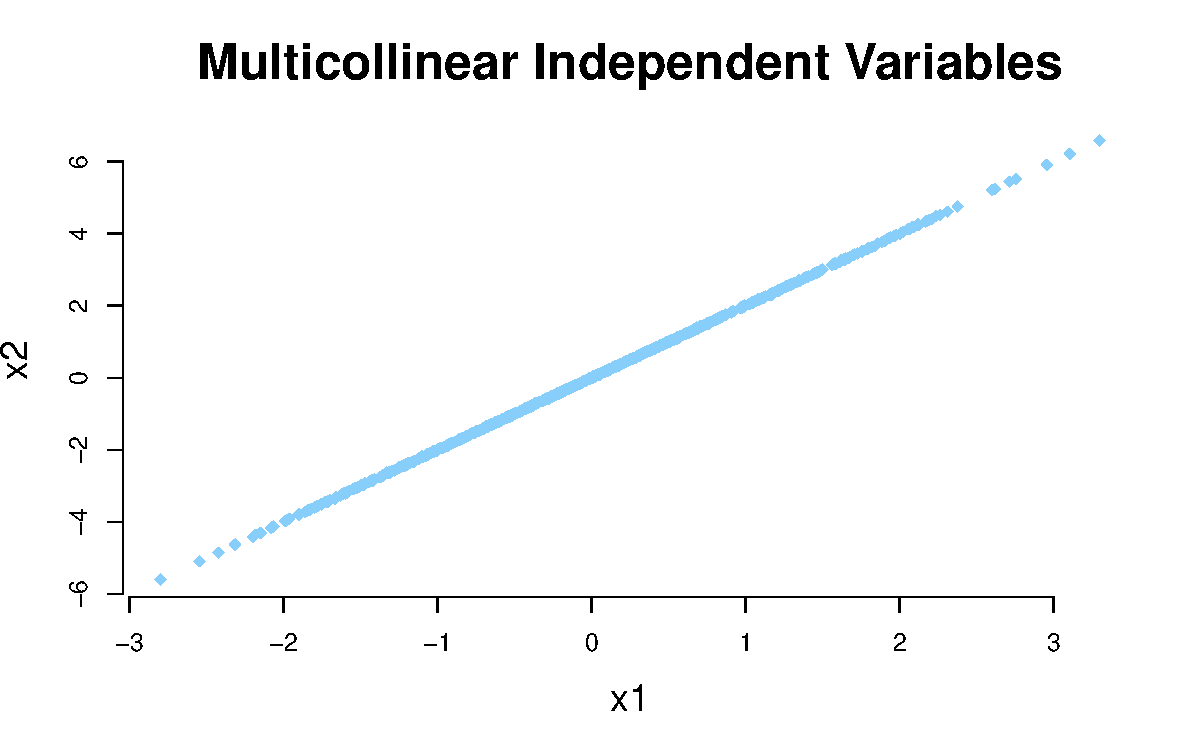
\includegraphics[scale=0.35]{multicollinearity.pdf}
\end{center}
\end{column}
\end{columns}

\end{frame}

%@@@@@@@@@@@@@@@@@@@@@@@@@@@@@@@@@@@@@@@@@@@@@@@@@
\begin{frame}
\frametitle{Problem 2: Multicollinearity}

\begin{itemize}
\item True relationship between $y$ and $x$'s is:
\begin{align*}
y = 1 + 2x_1 - x_2 + \varepsilon;
\end{align*}
\item[]\color{white} Suppose we omit $x_2$:
\end{itemize}

% latex table generated in R 4.1.1 by xtable 1.8-4 package
% Wed Nov  2 10:37:14 2022
\begin{table}[ht]
\centering
\begin{tabular}{rrrrr}
  \hline
\hline
 & Estimate & Std. Error & t value & Pr($>$$|$t$|$) \\ 
  \hline
\hline
(Intercept) & 1.0314 & 0.0314 & 32.88 & 0.0000 \\ 
  x1 & -4.2018 & 6.2780 & -0.67 & 0.5035 \\ 
  x2 & 2.0998 & 3.1390 & 0.67 & 0.5037 \\ 
   \hline
\hline
\end{tabular}
\end{table}
\end{frame}

%@@@@@@@@@@@@@@@@@@@@@@@@@@@@@@@@@@@@@@@@@@@@@@@@@
\begin{frame}
\frametitle{Problem 3: Heterscedasticity}

\begin{columns}
\begin{column}{0.5\textwidth}

\begin{itemize}
\item \textbf{Heterscedasticity} $=$ the standard deviation of the noise is not constant;
\bigskip
\bigskip

\item \textbf{Effect}: the $p$-values will be too large leading you to fail to reject the null when you really should;
\bigskip
\bigskip

\item \textbf{Fix}: transform variables (e.g. log $y$), advanced techniques.

\end{itemize}

\end{column}
\begin{column}{0.5\textwidth}
\begin{center}
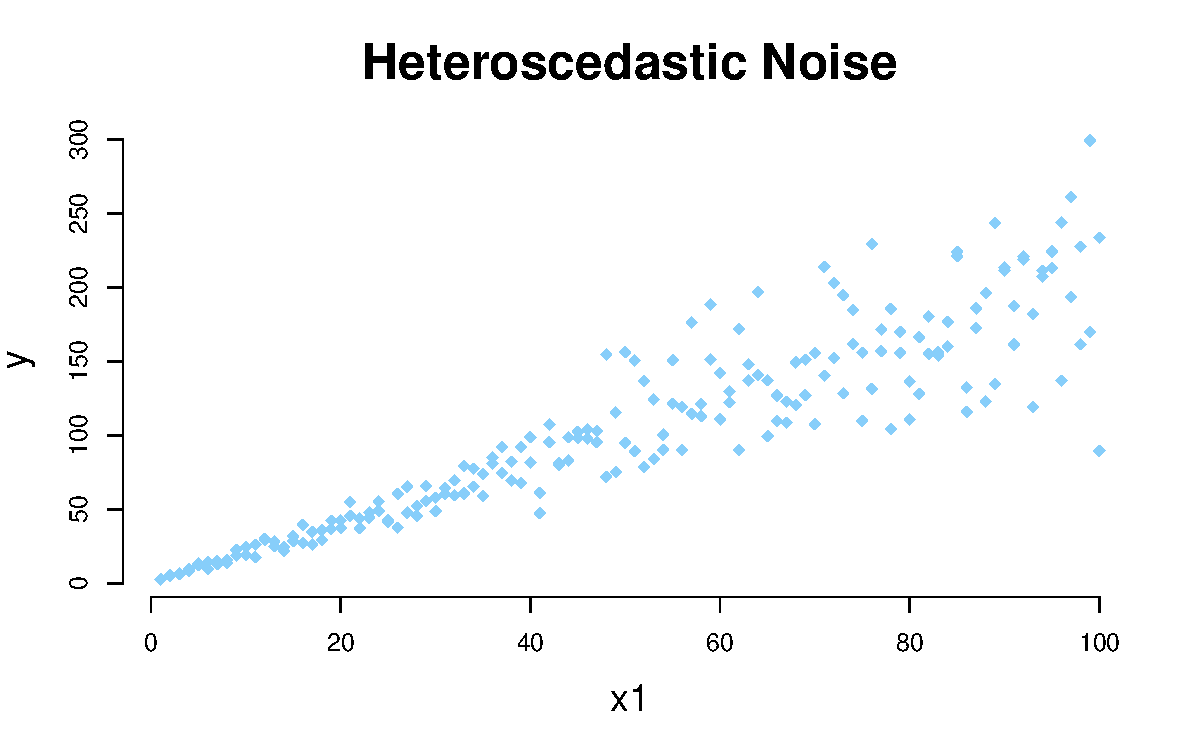
\includegraphics[scale=0.35]{heteroscedasticity.pdf}
\end{center}
\end{column}
\end{columns}


\end{frame}

%@@@@@@@@@@@@@@@@@@@@@@@@@@@@@@@@@@@@@@@@@@@@@@@@@
\begin{frame}
\frametitle{Problem 3: Heterscedasticity}

\begin{itemize}
\item True relationship between $y$ and $x$'s is:
\begin{align*}
y = 1 + 2x_1 - x_2 + \varepsilon;
\end{align*}
\item[]\color{white} Suppose we omit $x_2$:
\end{itemize}

% latex table generated in R 4.1.1 by xtable 1.8-4 package
% Wed Nov  2 10:49:19 2022
\begin{table}[ht]
\centering
\begin{tabular}{rrrrr}
  \hline
  \hline
 & Estimate & Std. Error & t value & Pr($>$$|$t$|$) \\ 
  \hline
    \hline
(Intercept) & 0.6148 & 3.8241 & 0.16 & 0.8724 \\ 
  x1 & 2.0667 & 0.0658 & 31.43 & 0.0000 \\ 
  x2 & -0.3911 & 1.8852 & -0.21 & 0.8359 \\ 
   \hline
      \hline
\end{tabular}
\end{table}

\end{frame}

%@@@@@@@@@@@@@@@@@@@@@@@@@@@@@@@@@@@@@@@@@@@@@@@@@
\begin{frame}
\frametitle{Problem 4: Measurement error}

\begin{itemize}
\item \textbf{Measurement error} $=$ we make mistakes measuring the independent variables when collecting the data;
\bigskip
\bigskip

\item \textbf{Effect}: the independent variable effect (the $\beta$) on the badly measured variable that linear regression estimates will be too small;
\bigskip
\bigskip

\item \textbf{Fix}: advanced techniques.

\end{itemize}

\end{frame}

%@@@@@@@@@@@@@@@@@@@@@@@@@@@@@@@@@@@@@@@@@@@@@@@@@
\begin{frame}
\frametitle{Problem 4: Measurement error}

\begin{itemize}
\item True relationship between $y$ and $x$'s is:
\begin{align*}
y = 1 + 2x_1 - x_2 + \varepsilon;
\end{align*}
\item When we collect the data we make mistakes in measuring so that we collect $x_2 + e$;
\end{itemize}

% latex table generated in R 4.1.1 by xtable 1.8-4 package
% Wed Nov  2 10:53:31 2022
\begin{table}[ht]
\centering
\begin{tabular}{rrrrr}
  \hline
  \hline
 & Estimate & Std. Error & t value & Pr($>$$|$t$|$) \\ 
  \hline
    \hline
(Intercept) & 1.4749 & 0.0361 & 40.89 & 0.0000 \\ 
  x1 & 2.0239 & 0.0327 & 61.87 & 0.0000 \\ 
  x2 & -0.9011 & 0.0306 & -29.43 & 0.0000 \\ 
   \hline
      \hline
\end{tabular}
\end{table}

\end{frame}

%@@@@@@@@@@@@@@@@@@@@@@@@@@@@@@@@@@@@@@@@@@@@@@@@@
\begin{frame}
\frametitle{Problem 4: Measurement error}

\begin{itemize}
\item True relationship between $y$ and $x$'s is:
\begin{align*}
y = 1 + 2x_1 - x_2 + \varepsilon;
\end{align*}
\item When we collect the data we make mistakes in measuring so that we collect $x_2 + e$;
\end{itemize}

% latex table generated in R 4.1.1 by xtable 1.8-4 package
% Wed Nov  2 10:57:22 2022
\begin{table}[ht]
\centering
\begin{tabular}{rrrrr}
  \hline
  \hline
 & Estimate & Std. Error & t value & Pr($>$$|$t$|$) \\ 
  \hline
    \hline
(Intercept) & 1.7834 & 0.0469 & 38.05 & 0.0000 \\ 
  x1 & 1.9934 & 0.0369 & 54.09 & 0.0000 \\ 
  x2 & -0.7493 & 0.0312 & -23.98 & 0.0000 \\ 
   \hline
      \hline
\end{tabular}
\end{table}

\end{frame}

%@@@@@@@@@@@@@@@@@@@@@@@@@@@@@@@@@@@@@@@@@@@@@@@@@
\begin{frame}
\frametitle{Problem 4: Measurement error}

\begin{itemize}
\item True relationship between $y$ and $x$'s is:
\begin{align*}
y = 1 + 2x_1 - x_2 + \varepsilon;
\end{align*}
\item When we collect the data we make mistakes in measuring so that we collect $x_2 + e$;
\end{itemize}

% latex table generated in R 4.1.1 by xtable 1.8-4 package
% Wed Nov  2 10:58:24 2022
\begin{table}[ht]
\centering
\begin{tabular}{rrrrr}
  \hline
  \hline
 & Estimate & Std. Error & t value & Pr($>$$|$t$|$) \\ 
  \hline
    \hline
(Intercept) & 1.9629 & 0.0581 & 33.81 & 0.0000 \\ 
  x1 & 1.9710 & 0.0385 & 51.22 & 0.0000 \\ 
  x2 & -0.6529 & 0.0293 & -22.28 & 0.0000 \\ 
   \hline
      \hline
\end{tabular}
\end{table}

\end{frame}

%@@@@@@@@@@@@@@@@@@@@@@@@@@@@@@@@@@@@@@@@@@@@@@@@@
\begin{frame}
\frametitle{Problem 4: Measurement error}

\begin{itemize}
\item True relationship between $y$ and $x$'s is:
\begin{align*}
y = 1 + 2x_1 - x_2 + \varepsilon;
\end{align*}
\item When we collect the data we make mistakes in measuring so that we collect $x_2 + e$;
\end{itemize}

% latex table generated in R 4.1.1 by xtable 1.8-4 package
% Wed Nov  2 10:59:53 2022
\begin{table}[ht]
\centering
\begin{tabular}{rrrrr}
  \hline
  \hline
 & Estimate & Std. Error & t value & Pr($>$$|$t$|$) \\ 
  \hline
    \hline
(Intercept) & 1.7451 & 0.0745 & 23.43 & 0.0000 \\ 
  x1 & 2.0534 & 0.0397 & 51.72 & 0.0000 \\ 
  x2 & -0.3123 & 0.0245 & -12.72 & 0.0000 \\ 
   \hline
      \hline
\end{tabular}
\end{table}

\end{frame}

%@@@@@@@@@@@@@@@@@@@@@@@@@@@@@@@@@@@@@@@@@@@@@@@@@
\begin{frame}
\frametitle{Problem 5: Endogeneity}

\begin{itemize}
\item \textbf{Endogeneity} $=$ the independent variables cause the dependent variable AND the dependent variable also causes one of the independent variables;
\bigskip
\bigskip

\item \textbf{Effect}: the independent variable effects (the $\beta$s) that linear regression estimates will be wrong;
\bigskip
\bigskip

\item \textbf{Fix}: theorizing about variable relationships, restructuring the data, removing independent variables thought to be caused by the dependent variable from the regression, advanced techniques.

\end{itemize}

\end{frame}

%@@@@@@@@@@@@@@@@@@@@@@@@@@@@@@@@@@@@@@@@@@@@@@@@@
\begin{frame}
\frametitle{Problem 5: Endogeneity}

\begin{itemize}
\item True relationship between $y$ and $x$'s is:
\begin{align*}
y &= 1 + 2x_1 - x_2 + \varepsilon;\\
x_ 2 &= 3y + e;
\end{align*}
\end{itemize}

% latex table generated in R 4.1.1 by xtable 1.8-4 package
% Wed Nov  2 11:03:22 2022
\begin{table}[ht]
\centering
\begin{tabular}{rrrrr}
  \hline
  \hline
 & Estimate & Std. Error & t value & Pr($>$$|$t$|$) \\ 
  \hline
    \hline
(Intercept) & 0.0244 & 0.0101 & 2.42 & 0.0155 \\ 
  x1 & 0.0647 & 0.0107 & 6.07 & 0.0000 \\ 
  x2 & 0.3017 & 0.0032 & 95.35 & 0.0000 \\ 
   \hline
      \hline
\end{tabular}
\end{table}

\end{frame}

%@@@@@@@@@@@@@@@@@@@@@@@@@@@@@@@@@@@@@@@@@@@@@@@@@
\begin{frame}

\begin{center}
\Huge\textbf{Why should we care?}\\
\bigskip
\bigskip
\large Linear regression -- so powerful...and so easy to mess up!\\
\end{center}

\end{frame}



\end{document}






